\begin{doublespace}

\chapter{Ecological and mutation-order speciation in digital organisms}
\label{chap:ecol_mo}



\section{Introduction}

Reproductive isolation between populations
often evolves as a byproduct of independent adaptation
to new environments \citep{coy04,sch09,sob10}.
%
When these environments' selective pressures are different,
divergent selection can cause populations
to acquire different, often incompatible, alleles.
%
This divergent process can generate reproductive isolation
both in nature \citep[reviewed in][]{run05,sch09}
and in laboratory experiments \citetext{\citealp{det07,det08};
reviewed in \citealp{ric93} and \citealp{fry09}}.
%
Complete reproductive isolation due to this process
is known as `ecological speciation' \citep{sch09}.
%
On the other hand, if the environments' selective pressures
are similar or identical (parallel or uniform selection),
populations may diverge genetically
by the chance fixation of different alleles.
%
Although laboratory experiments and theoretical studies suggest that
such process may lead to `mutation-order speciation' \citep{sch09,nos11},
its effectiveness in generating reproductive isolation
compared to ecological speciation is unknown.



The main purpose of this study is to directly compare
the strength of reproductive isolation
generated by ecological and mutation-order processes.
%
Specifically, we measure both the degree of postzygotic isolation
(i.e., hybrid inviability)
as well as the amount of genetic divergence between populations
evolved under either different environments or the same environments.
%
Because there is a higher chance of parallel evolution
when environments are similar \citep{sch09b},
we expect that postzygotic isolation and genetic divergence
under a mutation-order process will be weaker than under an ecological process.



We also examine the effect of migration
on both ecological and mutation-order processes.
%
Migration between populations increases the chance of gene flow,
which often slows genetic (and thus adaptive) divergence,
although gene flow can also promote divergence \citep{gar06,ras08}.
%
We vary the amount of migration between populations
under both ecological and mutation-order processes,
from allopatry to sympatry.
%
We expect that migration will have a stronger negative effect
on the evolution of reproductive isolation under mutation-order scenarios
because, under uniform selection, an adaptive mutation
that arises in one population is also selectively
favored in the other \citep{sch09,nos09b,nos11}.



We also examine how the environments' dimensionality
(i.e., number of selective pressures)
affects the strength of reproductive isolation
for both ecological and mutation-order processes.
%
In high-dimensional environments,
there are more opportunities for populations
to adapt in different ways \citep{ric93,nos09},
which may lead to stronger reproductive isolation
for both ecological and mutation-order processes.
%
High dimensionality, however, may also constrain speciation
when trade-offs among adaptive traits hinder adaptation
and therefore decrease the probability of reproductive isolation.



Finally, we examine one possible cause for differences
in hybrid fitness between ecological and mutation-order processes.
%
As populations adapt to their local environments independently,
there is no guarantee that alleles acquired in one population
will interact positively, or even neutrally, in the hybrid
with alleles acquired in the other population \citep{coy04}.
%
Negative interactions between alleles from two populations
are known as Dob\-zhan\-sky-Mul\-ler incompatibilities (DMIs),
and both ecological and mutation-order process
may cause them to form and thus lead to postzygotic isolation \citep{sch09}.
%
It is unknown, however, whether ecological or mutation-order speciation
differ in their propensity to produce DMIs.
%
Although a mutation-order process may be expected to have
fewer DMIs initially than an ecological process
because uniform selection selects for the same alleles,
such expectation diminishes the more populations diverge \citep{sch09}.



In this study, we use the software Avida (see p. \pageref{sec:avida}
to carry out our experiments.
%
Avida \citep{ofr04} is an artificial life research platform
where digital organisms evolve due to genetic variation, inheritance,
and differential reproduction (see Methods).
%
Avida has been used previously
in a wide range of ecological and evolutionary studies
\citep[e.g.,][]{len03,cho04,ele07,ost07,mis10}.
%
There are several reasons for using digital organisms to study evolution:
we can observe millions of generations in a few days,
conduct hundreds of replicate experiments,
easily manipulate genomes,
and accurately measure fitness.
%
Digital organisms in Avida are not meant to specifically mimic
the details of real biological organisms.
%
Instead, digital organisms have a unique genetic system (see Methods).
%
Despite these differences, the general principles
that make evolution possible are still the same,
which allows Avida to be used to test the generality
of evolutionary theories and hypotheses.
%
Indeed, several evolutionary properties
have been found to be remarkably similar to that of biological organisms
\citep{wil02,ada06}
(e.g., the distribution of mutational effects, the types of epistasis,
and the genetic architecture of sexual organisms).
%
Digital organisms improve on simple two-locus models of speciation
because in Avida, traits are complex,
involving multiple loci and epistatic interactions among alleles \citep{len99}.



\section{Methods}

\subsection{Experimental design}

The Avida configuration files used to run our experiments
are available in the Dryad Data Repository.
%
To generate the ancestral population,
we founded a population with an organism that could replicate
but could not perform any tasks.
%
We then let this population evolve under the default nine-task environment
for 500,000 updates ($\sim$~42,000 generations).
%
An `update' is a measurement of time in Avida, increasing by one each time
organisms execute 60 instructions (on average).
%
For the evolution of the ancestral population,
we set the maximum population size to 10,000 individuals.
%
The length of the genome was set to 200 instructions,
and to ensure homologous recombination
during sexual reproduction, the genome length was fixed.
%
The mutation rate was set to 0.1 mutations per genome per generation.



We then set up four treatments (described below), which we call
`drift,' `ecological,' `mu\-ta\-tion-or\-der 1,' and `mu\-ta\-tion-or\-der 2.'
%
For each treatment,
the population size was set to 2,000 individuals
and divided into two demes, each of size 1,000.
%
In the drift treatment, both demes' environments
were the same as the ancestral (environment `A').
%
For each remaining treatments,
we set up two subtreatments (described below):
low dimensionality and high dimensionality.
%
For this study, dimensionality refers to the number of tasks
for which that environment rewards organisms for performing such tasks.
%
In the ecological treatment, the demes' environments
were different from each other and different from the ancestral
(environments `1L' and `2L' for low dimensionality
and environments `1H' and `2H' for high dimensionality).
%
In the mutation-order 1 treatment,
the demes' environments were the same as each other
but different from the ancestral
(environment `1L' for low dimensionality
and environment `1H' for high dimensionality).
%
Similarly, in the mutation-order 2 treatment,
the demes' environments were the same as each other
but different from the ancestral
(environment `2L' for low dimensionality
and environment `2H' for high dimensionality).



The specific tasks that were rewarded in each environment
remained the same for the rest of this study.
%
The number of tasks for the low and high environments
were chosen as two extremes: two tasks for low dimensionality
and the maximum of 34 (i.e., 68 possible tasks divided randomly
into two demes) for high dimensionality.
%
The specific tasks for environments 1L and 2L were chosen at random
from tasks that were known to evolve within 10,000 updates in preliminary runs.
%
Environments 1L and 2L shared no tasks;
similarly, environments 1H and 2H shared no tasks.
%
The specific tasks rewarded in each environment
are part of the Avida configuration files,
which are available in the Dryad Data Repository.



Each treatment was replicated 20 times
with a different random sample of 2,000 organisms (1,000 per deme)
from the ancestral population.
%
Successive random samples were reused for each treatment,
so that the genotypes in replicate $n$ of a treatment
were the same as the genotypes in replicate $n$ of another treatment.
%
We ran each replicate for 10,000 updates ($\sim$~850 generations).
%
For each run, the entire population of organisms
was saved every 100 updates ($\sim$~8.5 generations).
%
To examine the effect of gene flow,
each replicate was run under eight migration rates
(for the entire length of the run):
0.0 (allopatry), 0.00001, 0.0001, 0.001, 0.01, 0.05, 0.1, and 0.5 (sympatry).
%
Migration rate is the probability of an offspring
being born in a deme different than its parents;
the migrating offspring was placed in a random
location in the other deme (i.e., there were no hybrid zones)
but the parents remained in their own demes.
%
In all, there were 1,120 runs.



We measured the overall strength of selection in each environment
(1L, 2L, 1H, and 2H) at the end of each `ecological' replicate run.
%
First, for every organism in a population that could perform at least one task,
we counted the number of tasks it could perform
and calculated its fitness relative to the mean.
%
We then used linear regression on the relationship between
the number of tasks an organism could perform and its relative fitness.
%
The slope of this line is the strength of selection \citep{con04}.
%
We report these results here, as they are part of the environment
in which populations evolved.
%
For environments 1L and 2L, the mean strengths of selection were
0.3440 (0.3375--0.3562, 95\% bootstrap C.I.) and 0.3353 (0.3341--0.3366),
respectively.
%
For environments 1H and 2H, the mean strengths of selection were
0.2045 (0.1852--0.2248) and 0.1899 (0.1762--0.2041), respectively.
%
We discuss the strength of selection in the Discussion.



\subsection{Postzygotic reproductive isolation}

In this study,
we focus on the evolution of postzygotic reproductive isolation.
%
To measure the strength of postzygotic isolation for each treatment,
we first selected 1,000 random pairs of organisms (one from each deme)
and created one hybrid per pair at the end of each replicate run.
%
We then calculated the fitness of each hybrid
as the mean fitness relative to each parent.
%
Finally, we compared the mean hybrid fitnesses for each treatment---%
the lower this fitness, the stronger the isolation.
%
Note that hybrids were created
after the experiments were finished;
no hybrids were put back into the population.



Two types of hybridizations were performed for creating hybrids
after the populations had evolved.
%
The first followed the method used in Avida for sexual reproduction
(and the way in which all our experimental populations experienced):
a randomly-sized genomic region starting at a random locus was chosen
(both random numbers came from a uniform distribution),
and two recombinant offspring were created by exchanging
the genetic region of one parent with the other (two-point crossover).
%
We randomly chose one of the two offspring as the hybrid.
%
We also performed a more fine-scaled hybridization method,
where each locus of a hybrid had the same probability (0.5)
of it coming from either one or the other parent.
%
This method effectively increased the number of crossover points up to 200
and the number of regions that can be exchanged up to 100.
%
We used this multiple-point crossover method
to break apart coadapted gene complexes,
following the same logic that researchers
use when carrying out parental backcrosses
or intercrosses between hybrids \citep[e.g.,][]{li97,bur99}.
%
Multiple crossover points can expose
incompatible gene complexes between species,
revealing patterns of divergence
that would be difficult to detect with
recombination at only two crossover points.



\subsection{Genetic divergence}



To quantify the homogenizing effects of gene flow,
we calculated the genetic divergence
between each replicate pair of demes
under 0.0 and 0.01 migration for each treatment.
%
Genetic divergence was measured as the fixation index
$F_{\mathrm{ST}} = 1 - H_{\mathrm{S}} / H_{\mathrm{T}}$,
where $H_{\mathrm{S}}$ is the mean heterozygosity of each deme
and $H_{\mathrm{T}}$ is the heterozygosity of both demes
treated as one population \citep[p. 118]{har97}.
%
The heterozygosity of a deme
is the mean heterozygosity at all loci.
%
The heterozygosity at a locus is $H = 1 - \sum_{i = 1}^{n} x_i^{2}$,
where $n$ is the number of alleles segregating at that locus
and $x_i$ is the frequency of the $i$th allele \citep[p. 15]{gil04}.
%
$F_{\mathrm{ST}}$ values between 0 and 0.05
would indicate little or no genetic divergence
between two demes \citep[p. 118]{har97}.
%
We expect that under zero migration
$F_{\mathrm{ST}}$ values will be significantly higher
than those under the 0.01 migration rate.
%
Significance among treatments was determined by comparing their
95\% confidence intervals of the mean $F_{\mathrm{ST}}$.
%
Each confidence interval was estimated by calculating 10,000 means
of random samples (with replacement) of the $F_{\mathrm{ST}}$ values
from the 20 replicates
(i.e., each sample contained 20 $F_{\mathrm{ST}}$ values).
%
The interval between 2.5\% and 97.5\% of means defined the confidence interval.



To test whether gene flow causes the same mutations%
---specifically those involved in performing a task---%
to fix under mutation-order speciation,
we carried out a two-step process to identify and map such mutations.
%
First, to determine whether the fixed mutations in a deme
were necessary to perform a task,
we reverted each locus, one by one, of the deme's consensus sequence
to the ancestral state.
%
If any reversion eliminated the ability to perform a task,
then the allele at that locus must be important for that task.
%
We ignored loci in which a reversion caused
complete inviability of the organism,
as these loci were involved in more than just task performance.
%
Second, we aligned the consensus sequences of each pair of demes
under 0.0 and 0.01 migration and highlighted the mutations we found above.



\subsection{Hybrid phenotypes}

To examine a possible cause for differences
in hybrid fitness between ecological and mutation-order processes,
we counted the number of times that hybrids had low fitness
due to Dob\-zhan\-sky-Mul\-ler incompatibilities (DMIs).
%
Under two-point crossover recombination,
a hybrid is made up of two parental components,
which we call C$_{1}$ and C$_{2}$.
%
If C$_{1}$ or C$_{2}$ contains the instructions to perform a task
but the full hybrid cannot perform that task,
C$_{1}$ and C$_{2}$ must interfere with one another through at least one DMI.
%
To determine whether a hybrid had low fitness due to DMIs,
we constructed two genotypes by making two copies of the hybrid,
where we replaced C$_{2}$ in the first copy, and C$_{1}$ in the second copy,
with the corresponding ancestral genetic region.
%
In this way, we constructed two `component' genotypes,
where each parental component was isolated
in the genetic background of the ancestor.
%
We then determined the tasks that these component genotypes
as well as the original hybrid could perform.
%
If either component genotype could perform a task
but the hybrid could not, then at least one DMI was present
(Figure \ref{fig:hybrid_components}).
%
We performed this analysis on 1,000 hybrids per replicate
in both the ecological and mutation-order treatments
under zero migration, low dimensionality, and two-point crossover recombination.



\begin{figure}
\centering
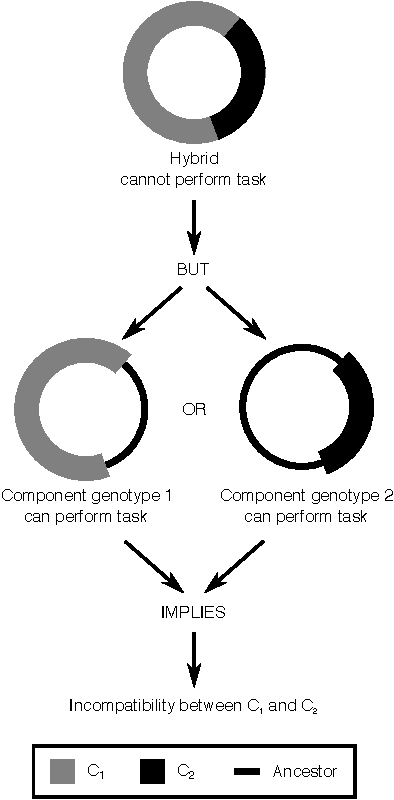
\includegraphics[width=3.5in]{hybrid_components.pdf}
\caption{Method to determine whether a hybrid contains
  genetic incompatibilities.
  %
  A hybrid is composed of two parental components, C$_{1}$ and C$_{2}$.
  %
  Note that a parental component is only the parental region
  inherited by the hybrid; it is not the complete parent.
  %
  If the hybrid cannot perform the task but either parental component can,
  then there must be at least one incompatibility between the components.}
\label{fig:hybrid_components}
\end{figure}



Because in this system an organism's fitness is largely determined
by the number and type of tasks it can perform (i.e., its phenotype),
we identified the tasks that could be performed by each hybrid
for both ecological and mutation-order processes.
%
Note that this analysis is independent of the environment
because an organism may have the ability to perform a task
even if the environment does not reward for it.
%
For simplicity, we focused only on
the zero migration, low dimensionality set of treatments
that were hybridized with a two-point crossover.
%
For the ecological treatment,
hybrids were categorized by the number tasks they could perform:
(`\mbox{0-0}')~no tasks in either environment,
(`\mbox{1-0}')~one task in one environment but none in the other,
(`\mbox{1-1}')~one task in each environment,
(`\mbox{2-0}')~two tasks in one environment but none in the other,
(`\mbox{2-1}')~two tasks in one environment and one in the other,
and (`\mbox{2-2}')~two tasks in both environments.
%
For the mutation-order treatment,
hybrids were categorized by the tasks they could perform:
(`None')~no tasks,
(`1')~task~1,
(`2')~task~2,
and (`1 and 2')~both tasks.
%
For those hybrids that could perform both tasks
in the mutation-order treatment,
we determined the tasks that each hybrid's parental components could perform.
%
We categorized these parental components as
(`0,0')~no parental component performs any task,
(`1,0')~one parental component performs one task but the other none,
(`1,1')~each parental component performs a different task,
and (`2,*')~at least one parental component performs both tasks.
%
This analysis will reveal the reason, at the phenotypic level,
for differences in hybrid performance between ecological
and mutation-order processes.
%
Four replicates from the ecological treatment,
one replicate from the mutation-order 1 treatment,
and six replicates from the mutation-order 2 treatment
were removed from the analysis above.
%
In the ecological treatment, the removed replicates contained parents
that could fortuitously perform a task of the other environment
(even though there was no selective pressure for that task),
and thus it would be unclear from which parent the task was inherited
by the hybrids.
%
In the mutation-order treatments, the removed replicates contained parents
that could not perform both tasks and, therefore, was the reason
that some of the hybrids were unfit.



\section{Results}

\subsection{Postzygotic reproductive isolation}

When hybrids between the evolved demes
were created by recombining a single genetic region (`two-point crossover'),
reproductive isolation between demes
that adapted to different environments (ecological treatment)
was considerably stronger than
reproductive isolation between demes
that adapted to the same environment (mutation-order treatment)
(Figs. \ref{hybrid_fitness}A and \ref{hybrid_fitness}B).
%
With zero migration, for instance,
reproductive isolation in the ecological treatment
was more than twice as strong than in the mutation-order treatment.
%
There was no reproductive isolation between demes
evolving neutrally in the ancestral environment (drift treatment):
the mean hybrid fitness was $>$~0.99 at all migration rates.



\begin{figure}
\centering
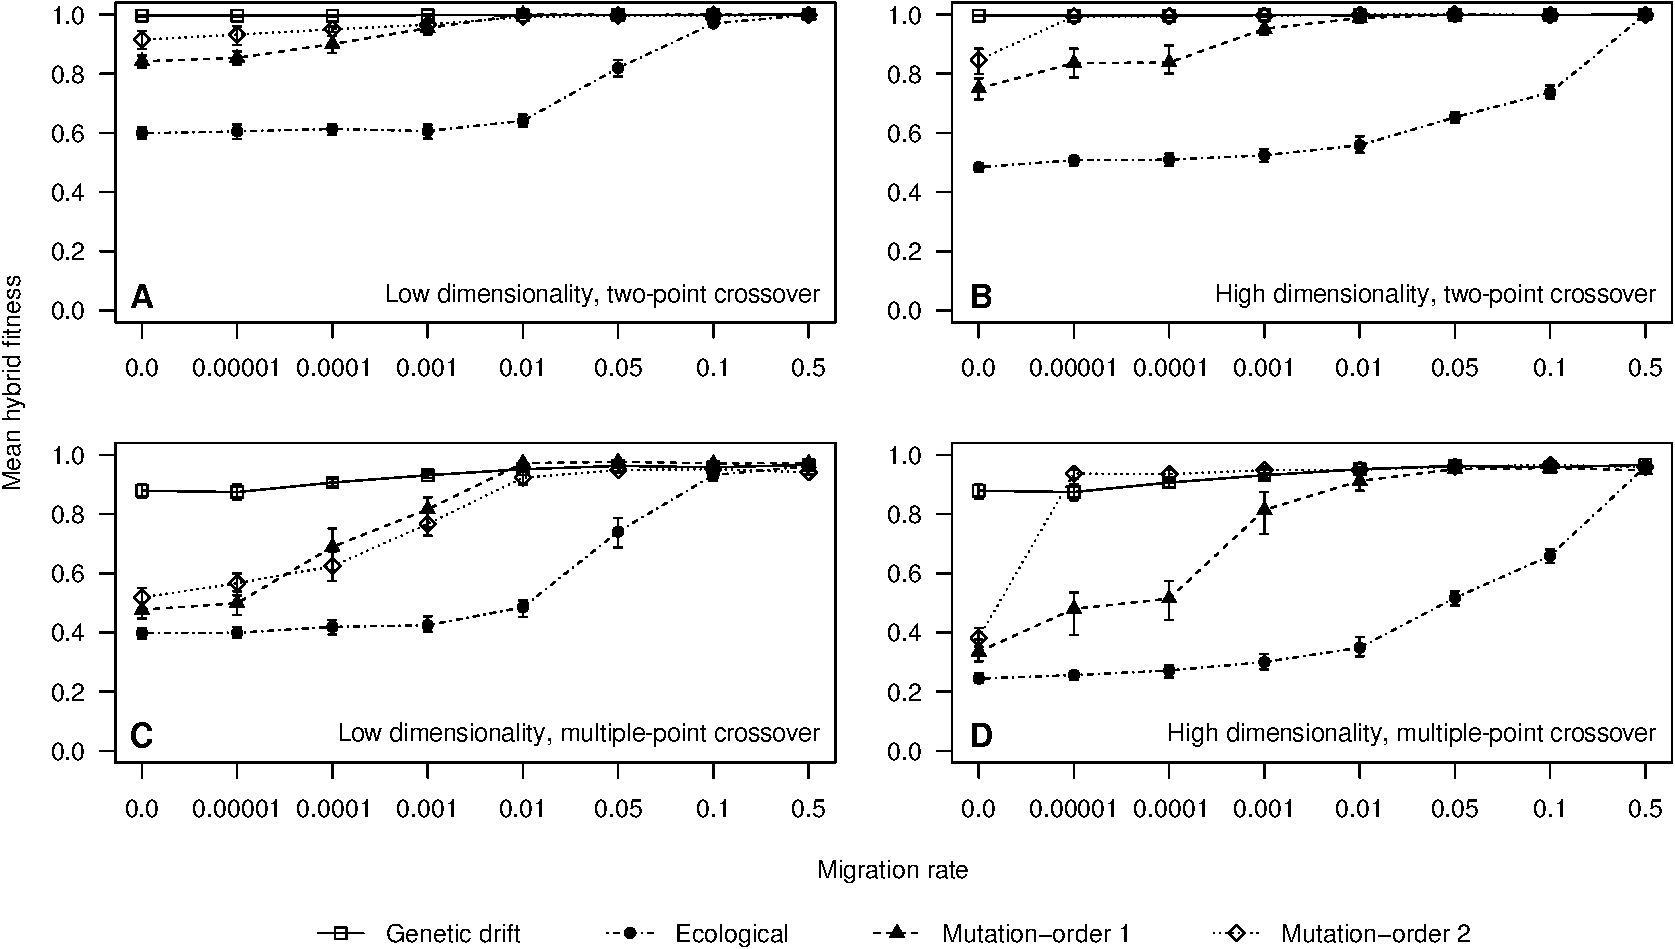
\includegraphics[width=0.95\linewidth]{hybrid_fitness.pdf}
\caption{Mean fitness of hybrids (y-axis)
  between populations evolved under various migration rates (x-axis)
  and different treatments (markers and lines):
  the ancestral environment (`Genetic drift'),
  different new environments (`Ecological'),
  or the same new environment (`Mutation-order 1' and `Mutation-order 2').
  At low dimensionality (A and C),
  the new environments rewarded only two tasks;
  at high dimensionality (B and D),
  the new environments rewarded 34 tasks.
  With two-point crossover (A and B),
  only one region was exchanged when creating hybrids;
  with multiple-point crossover (C and D),
  up to 100 regions were exchanged.}
\label{hybrid_fitness}
\end{figure}



Reproductive isolation in the mutation-order treatment
was more sensitive to gene flow than in the ecological treatment
(Figs. \ref{hybrid_fitness}A and \ref{hybrid_fitness}B).
%
At the 0.01 migration rate, for instance,
the mean hybrid fitness in the mutation-order treatment was $>$~0.98,
but in the ecological treatment reproductive isolation
was almost as strong as without migration.
%
The mutation-order 2 treatment was more sensitive to gene flow
than the mutation-order 1 treatment
(no reproductive isolation at a migration rate of 0.00001).



When the environment rewarded for many tasks (high dimensionality),
reproductive isolation was often stronger than
when the environment rewarded for only two tasks (low dimensionality)
(compare Figs. \ref{hybrid_fitness}A and \ref{hybrid_fitness}B,
Figs. \ref{hybrid_fitness}C and \ref{hybrid_fitness}D).
%
This pattern was most evident in the ecological treatment,
even at moderately high migration rates;
for example, the mean hybrid fitness in the ecological treatment
at 0.1 migration was 0.97 under low dimensionality
but only 0.74 under high dimensionality.
%
In the mutation-order treatments, however,
reproductive isolation under high dimensionality at migration rates $>$ 0
was not always stronger than under low dimensionality,
showing again that mutation-order was sensitive to gene flow.



When hybrids between the evolved demes
were created by recombining up to 100 genetic regions
(`multiple-point crossover'),
reproductive isolation in the ecological and mutation-order treatments
was stronger (Figs. \ref{hybrid_fitness}C and \ref{hybrid_fitness}D).
%
Note that recombination with multiple crossover points was used only
to create hybrids for the calculation of postzygotic isolation;
all populations were evolved under two-point crossover recombination.
%
The mean hybrid fitness with multiple-point crossover
was significantly lower than that with two-point crossover,
dropping 33\% and 48\% in the ecological treatment
for low and high dimensionality (respectively)
and 53\% and 43\% in the mutation-order treatments.
%
The difference in strengths of reproductive isolation
between ecological and mutation-order treatments
was now smaller than that with two-point crossover.
%
Reproductive isolation in the mutation-order treatment
remained more sensitive to gene flow than in the ecological treatment.
%
Reproductive isolation in the genetic drift treatment with little migration
was significantly greater than with two-point crossover.
%
Interestingly, reproductive isolation in the genetic drift treatment
with 0.00001 migration and high dimensionality
was even greater than in the mutation-order 2 treatment.



\subsection{Genetic divergence}

The genetic divergence under zero migration was significantly higher
than that under 0.01 migration for all treatments (Table \ref{tbl_fst}),
demonstrating that gene flow between populations had a homogenizing effect.
%
Under 0.01 migration, the mutation-order treatments had little genetic
divergence ($F_{\mathrm{ST}} <$ 0.05), which was significantly lower than the
ecological treatments, suggesting that the mutation-order treatments were more
sensitive to gene flow than the ecological treatments.
%
Interestingly, the drift treatment under zero migration showed high levels of
genetic divergence, as high as the ecological and mutation-order treatments for
low dimensionality.
%
Under zero migration, the genetic divergence for each treatment for high
dimensionality was significantly higher than those for low dimensionality.
%
Under 0.01 migration, the genetic divergence for the ecological treatment for
high dimensionality was significantly higher than that for low dimensionality,
but for the mutation-order treatments there was no difference in the genetic
divergence between low and high dimensionalities.
%
In agreement with these results,
the sequences for each pair of demes for treatments
under zero migration did not align as well as those
under 0.01 migration (Fig. \ref{task_muts}).
%
These result suggest that the reason that reproductive isolation
was mostly absent under a mutation-order process with gene flow
is that the key mutations that allowed organisms to perform tasks were the same
(i.e., no genetic divergence for task-related mutations).



\begin{table}
\centering
\caption{Genetic divergence ($F_{\mathrm{ST}}$)
  between demes for each treatment.}
\begin{tabular}{llcc}
\cline{3-4}
  & & \multicolumn{2}{c}{Migration rate} \\
\hline
Dimensionality & Treatment & 0.0 & 0.01 \\
\hline
--  & Drift            & 0.3136$^{a}$ & 0.0187$^{b}$ \\
\hline
Low & Ecological       & 0.3173$^{a}$ & 0.1387$^{c}$ \\
Low & Mutation-order 1 & 0.3096$^{a}$ & 0.0186$^{b}$ \\
Low & Mutation-order 2 & 0.3002$^{a}$ & 0.0216$^{b}$ \\
\hline
High & Ecological       & 0.4187$^{d}$ & 0.2680$^{e}$ \\
High & Mutation-order 1 & 0.4221$^{d}$ & 0.0304$^{b}$ \\
High & Mutation-order 2 & 0.3758$^{f}$ & 0.0199$^{b}$ \\
\hline
\multicolumn{4}{p{4in}}{\small\emph{Note:} Shared superscript letters indicate
  that those values are not significantly different
  (95\% bootstrap confidence interval).}
\end{tabular}
\label{tbl_fst}
\end{table}



\begin{figure}
\centering
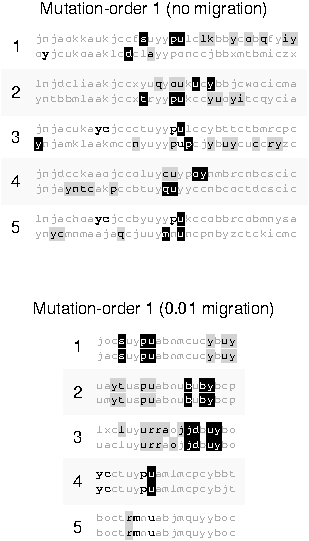
\includegraphics[height=5in]{task-muts.pdf}
\caption{Consensus sequences of the first five evolved replicate pairs of demes
  in the mutation-order~1 treatment under zero migration (top)
  and 0.01 migration (bottom).
  %
  Similar results were observed for the mu\-ta\-tion-order~2 treatment.
  %
  Sequences were 200 instructions in length,
  but only the loci that differed among
  each set of five replicates are shown.
  %
  Derived alleles involved in performing a task are highlighted
  (black highlight~=~task~1, gray highlight~=~task~2, bold font~=~both).}
\label{task_muts}
\end{figure}



\subsection{Hybrid phenotypes}

In the ecological treatment,
we found that each replicate had, on average,
268.3 hybrids (218.0--315.8, 95\% bootstrap mean C.I.) of 1,000
that contained at least one DMI between their parental components.
%
In the mutation-order treatments,
this quantity was 77.1 (45.8--111.2) and 128 (83.5--176.5) of 1,000.
%
Therefore, populations that adapted to different environments
accumulated more DMIs than populations that adapted to similar environments.



Because hybrids, on average, inherit half the genome of each parent,
we expected that hybrids, on average, would inherit half the tasks
from each parent (here we focused on the treatments without migration,
low dimensionality, and two-point crossover).
%
In the ecological treatment, we found that hybrids were more likely to perform
zero, one, or two tasks from one parent and none from the other
(Figure \ref{hybrid_counts}A).
%
Less than 10\% of hybrids were able to perform all four tasks.
%
For the mutation-order treatments,
most hybrids could perform both tasks
(Figure \ref{hybrid_counts}B and \ref{hybrid_counts}C),
but because the parents could also perform both tasks,
this information alone did not tell whether hybrids inherited
one task from each parent or some other combination.
%
When we analyzed those hybrids that could perform both tasks,
we found that most inherited both tasks from just one parent
(Figure \ref{fit_hybrid_components}),
although for mutation-order 2
the difference between those
that performed one task from each parent
and those that performed both tasks from one parent
was not significant.
%
Surprisingly, for the mutation-order 1 treatment
there were many hybrids that were fit
even though their parental components
could perform no tasks or just one task
(Figure \ref{fit_hybrid_components}A).



\begin{figure}
\centering
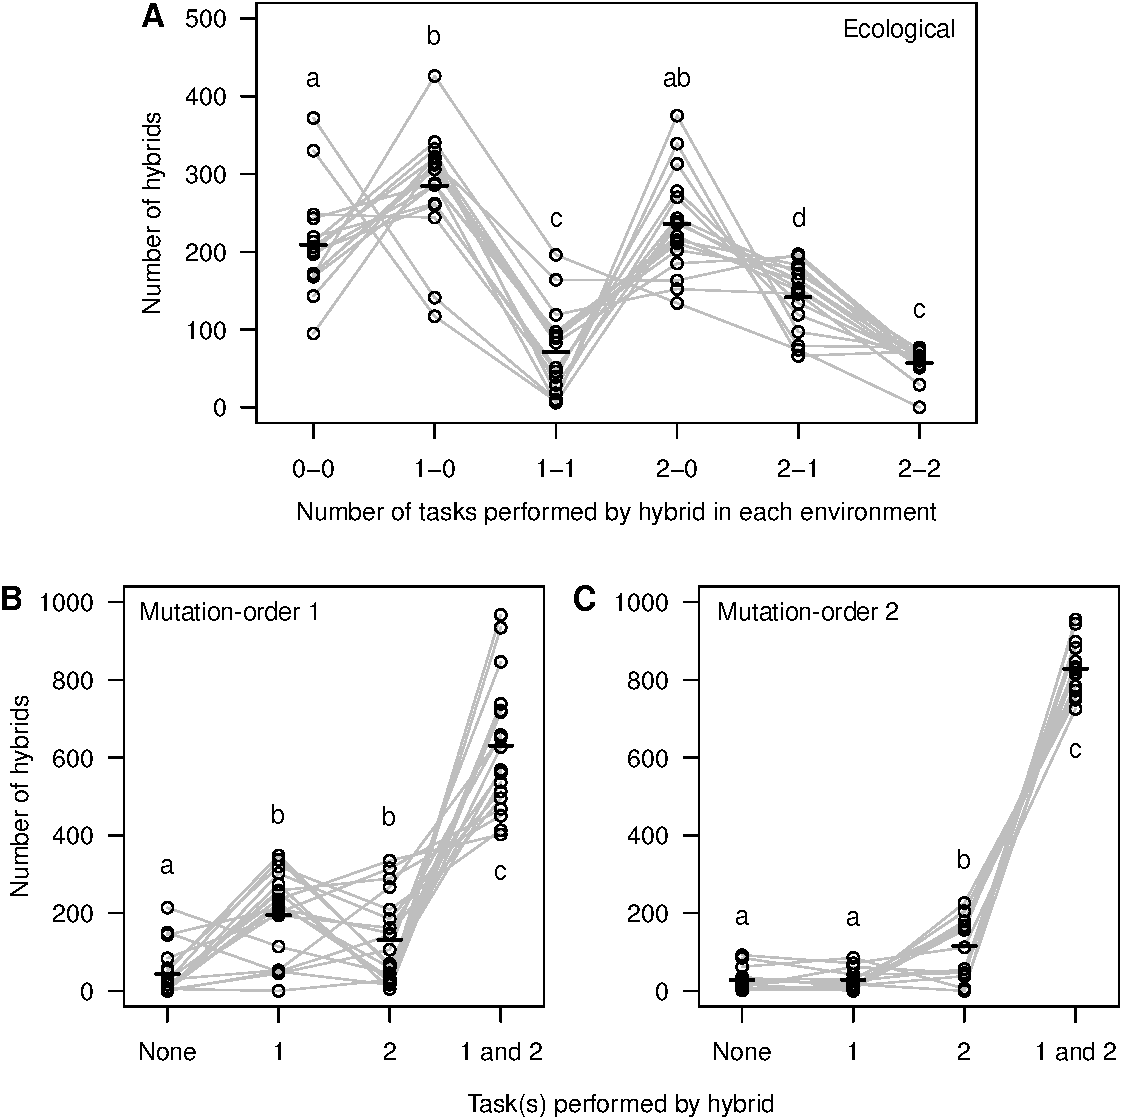
\includegraphics[width=0.95\linewidth]{hybrid_counts.pdf}
\caption{Number of hybrids able to perform certain tasks (see Methods) for
  the (A) ecological, (B) mutation-order-1, and (C) mutation-order-2 treatments
  under zero migration, low dimensionality, and two-point crossover.
  %
  Each point is a hybrid count (out of 1,000) for a single replicate.
  %
  Counts from the same replicate are connected by gray lines.
  %
  The mean hybrid count per category among replicates
  is indicated by a horizontal bar.
  %
  Non-significant differences between the mean hybrid counts
  share the same letter above (or below) the points in each category.}
\label{hybrid_counts}
\end{figure}



\begin{figure}
\centering
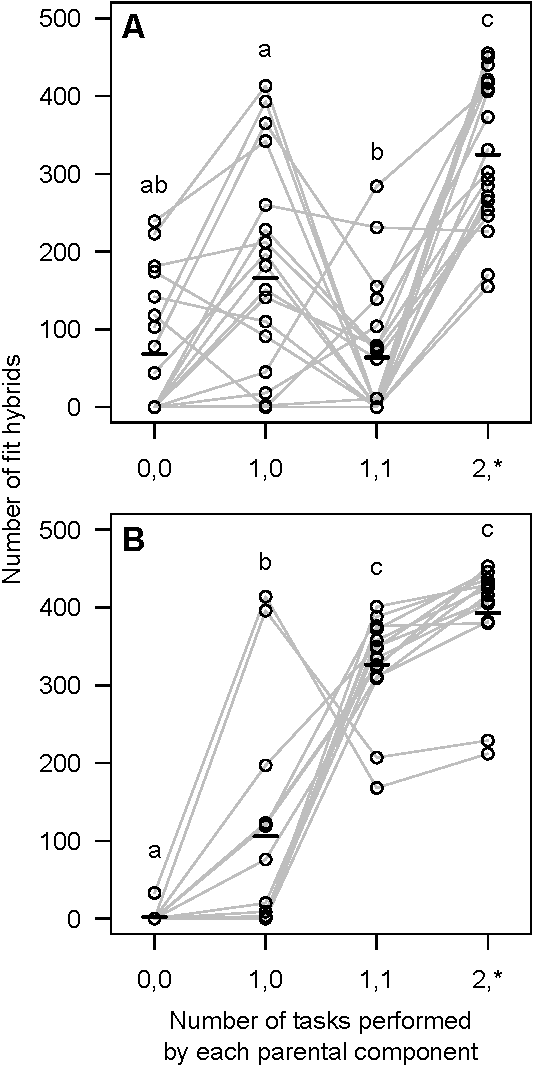
\includegraphics[width=0.95\linewidth]{fit_hybrid_components.pdf}
\caption{Number of fit hybrids (i.e., can perform two tasks)
  whose parental components can perform certain tasks (see Methods)
  for the (A) mutation-order 1 and (B) mutation-order 2 treatments
  under zero migration, low dimensionality, and two-point crossover.
  %
  Each point is a hybrid count for a single replicate.
  %
  Counts from the same replicate are connected by gray lines.
  %
  The mean hybrid count per category among replicates
  is indicated by a horizontal bar.
  %
  Non-significant differences between the mean hybrid counts
  share the same letter above the points in each category.}
\label{fit_hybrid_components}
\end{figure}



\section{Discussion}

In this study, we used experimental evolution of digital organisms
to compare the strength of postzygotic reproductive isolation
generated by ecological and mutation-order processes.
%
We assessed the strength of postzygotic isolation
by measuring the mean hybrid fitness relative to each parent
in its native environment.
%
We found that, using a two-point crossover recombination method,
the mean hybrid fitness was around 55\% under ecological divergence
but around 83\% under a mutation-order process.
%
Other studies have also found that the mean hybrid fitness
is lower under divergent selection than under parallel selection.
%
\citet{det07} found that the mean relative fitness of hybrids
between yeast populations evolved in different environments
(high-salinity and low-glucose) was around 87\%,
but hybrids from populations evolved
under the same environmental conditions were as fit as their parents.
%
Similar patterns were found in a filamentous fungus by \citet{det08},
although in one of the parental environments
hybrids between populations under divergent selection
performed better than hybrids under parallel selection.
%
Along with these studies, our study supports
the view that ecological divergence causes
stronger reproductive isolation than a mutation-order process.



It has been suggested that gene flow during speciation
may be common \citetext{\citealt{coy04}, p. 112; \citealt{nos08}},
which requires that genetic divergence with gene flow be possible.
%
We found that a migration rate of 1\% was not enough to prevent
genetic divergence under an ecological process (Table \ref{tbl_fst}).
%
This finding supports the notion that it is possible for populations
under divergent selection in the face of gene flow to continue to diverge.
%
Under a mutation-order process, however, a migration rate of 1\%
was enough to prevent genetic divergence,
which suggests that mutation-order speciation
is more sensitive to gene flow than ecological speciation.
%
\cite{nos11} also found in their computer simulations
that genetic divergence under a mutation-order process
did not occur $>$~1\% gene flow.
%
One of the mutation-order treatments under high dimensionality
was even sensitive to a migration rate of 0.00001.
%
We speculate that in this treatment (corresponding to environment 2H),
there was one or more large-effect adaptive mutation(s) that,
when migrated to the other deme, spread quickly and homogenized the demes.
%
We conclude that different populations under parallel selective pressures
probably require almost complete isolation for divergence to occur.



Reproductive isolation between populations evolving in high-dimensional
environments has been predicted and observed to be stronger than in single or
low dimensional environments \citep{ric93,nos09,nos09b}.
%
In \emph{Timema} walking-stick insects, for example, reproductive isolation
showed a positive correlation with environmental dimensionality
\citep{nos08b,nos09b}; further examples are reviewed in \citet{nos09}.
%
Most empirical studies, however, rely on incomplete measures of dimensionality
(imagine the difficulty in accounting for all selective pressures in the field).
%
In this study, we were able to control precisely the number of selective
pressures for the low and high dimensionality treatments.
%
We found that under an ecological process, reproductive isolation was stronger
between populations in high-dimensional environments than in low dimensional
environments.
%
Under a mutation-order process, however, this pattern held only when no
migration occurred between populations, but when gene flow was allowed this
pattern went away.
%
Our results support previous findings that dimensionality matters for
ecological speciation but suggests that for mutation-order speciation with gene
flow, environmental dimensionality may not be as important.



This conclusion was also supported by our measurements of genetic divergence:
there was no difference in genetic divergence between low and high
dimensionality for the mutation-order treatments under some gene flow.
%
For the ecological treatment, however, the genetic divergence in high
dimensionality was higher than in low dimensionality and higher than the
mutation-order treatments, again showing that mutation-order treatments were
more sensitive to gene flow.
%
Interestingly, under zero migration the drift treatment (where mutations fixed
neutrally) was as high as the ecological and mutation-order treatments under
low dimensionality, suggesting that most of the divergence in the ecological
and mutation-order treatments was actually the result of neutral fixations and
few adaptive mutations.
%
Indeed, in post-hoc analyses we found that about 90\% of mutational differences
between these treatments were due to neutral fixations, not adaptive mutations.
%
Another result to note is that under zero migration, the ecological and
mutation-order treatments had about the same level of genetic divergence, which
is closer to our result with multiple-point crossover than two-point crossover,
suggesting that in some cases the amount of postzygotic reproductive isolation
and genetic divergence are decoupled.



This decoupling between reproductive isolation and genetic divergence
has been observed in biological populations \citep{ste09,mac12}.
%
In these studies, genetic divergence was not found to be a good predictor
of sexual dimorphism or assortative mating \citep{ste09,mac12}.
%
In some cases, genetically closely related species
were ecologically and phenotypically divergent;
in other cases, genetically distant species
were phenotypically and ecologically close \citep{ste09}.
%
One proposed reason for this decoupling
is that temporal changes in selection pressures
alter the way in which natural and sexual selection interact \citep{mac12}.
%
Although assortative mating was not present in our digital populations---%
there was no mechanism for mate choice---%
reproductive isolation could not be predicted
solely based on genetic divergence.
%
We speculate that the reason was due to the degree of incompatibility
between alleles for the different modes of speciation:
alleles between populations were not as incompatible
under a mutation-order process than under an ecological process.
%
Our results support the notion that reproductive isolation
is not directly caused by genetic divergence but is a byproduct
of processes that also affect genetic divergence \citep{per11}.
%
Therefore, in order to determine reproductive isolation between populations,
one cannot rely solely on their genetic divergence;
reproductive isolation should be measured directly.



Traits that are physically modular
are hardly broken apart by recombination,
hiding genetic incompatibilities
that may have formed between populations.
%
To determine whether genetic incompatibilities
had formed between our populations
but were hidden by the modularity of traits,
we re-created hybrids through time using multiple-point crossover recombination
rather than two-point crossover recombination.
%
In multiple-point crossover recombination,
each locus of a hybrid's genome had an equal probability
of coming from either parent;
in this way, modular traits could be broken apart by recombination.
%
We found that the strength of reproductive isolation
decreased for both ecological and mutation-order speciation,
such that mutation-order speciation
was almost as strong as ecological speciation (Figure \ref{hybrid_fitness}).
%
We even see some reproductive isolation in the drift treatment,
showing that incompatibilities also formed,
but at a much slower rate than speciation by natural selection.
%
These findings show that genetic incompatibilities
were hidden by the modularity of traits.
%
In other words, genetic incompatibilities that formed between populations
were not always seen in hybrids because two-point crossover recombination
did not break apart co-adapted gene complexes coding for a task.
%
We note that the genetic architecture of our populations
evolved under two-point crossover recombination,
not multiple-point crossover recombination,
and thus the modularity of traits
and formation of genetic incompatibilities
may be different under a different recombination method.



Part of the reason that hybrids were more unfit in the ecological treatment
than in the mutation-order treatment was that in the ecological treatment
more genetic incompatibilities (DMIs) formed between populations.
%
This result supports the view that genetic incompatibilities
are an important cause of ecological speciation \citep{run05}.
%
Another reason that hybrids were more unfit in the ecological treatment was
that for a hybrid to be fully fit it had to inherit both sets of tasks from
both parents (i.e., four tasks), whereas for the mutation-order treatment,
hybrids required only two tasks to be fit.
%
In the ecological treatment, most hybrids inherited either one one two tasks
from one parent and none from the other, and in the mutation-order treatments,
most hybrids inherited both tasks from one parent, although in the second
mutation-order treatment hybrids often inherited one task from each parent.



We found that the selection coefficients of adaptive alleles
in the low dimensionality environments were higher
than that in the high dimensionality environments.
%
An opposite trend may have made it difficult to know whether
it was higher dimensionality or stronger selection that resulted
in hybrids being less fit under high dimensionality than low dimensionality.
%
The smaller selection coefficients in the high dimensionality environments
may seem puzzling at first.
%
But given that each additional task an organism could perform gives it
an equal amount of merit, the higher the merit, the less an additional task
contributes to the total merit.
%
Therefore, the more tasks organisms can perform in the high dimensionality
environment, the less beneficial each one becomes (i.e., diminishing returns).
%
The strengths of selection in either environment are nevertheless high overall,
but it is not uncommon for selection to be high in new environments
\citep[e.g.,][]{len91,det07}.
%
Future studies could investigate how the strength of selection may affect
the strength of postzygotic isolation
by manipulating the selection coefficients in each environment.



In summary, we used the artificial life platform Avida, which allowed us to
precisely control the type of selection (divergent or uniform), to compare the
strength of reproductive isolation between ecological and mutation-order
speciation.
%
By accurately measuring the fitness of hybrids between populations, we showed
that ecological speciation formed stronger postzygotic isolation than
mutation-order speciation, although they were not so different when
recombination involved crossover at multiple points.
%
In addition, Avida allowed us to test various specific migration rates during
the evolution of population pairs, where we found that mutation-order
speciation was more sensitive to gene flow than ecological speciation.
%
We were also able to control the number of selection pressures in each
population, and we found that environments with high dimensionality formed
stronger reproductive isolation than those with low dimensionality.
%
These results support ideas brought up in the literature but which have been
difficult to test in biological organisms.
%
Avida provided a platform for us to test these ideas much more easily, and
although digital organisms are more simplistic than biological organisms, they
are a genetic system that evolves and speciates and therefore allows us to test
the generality of hypotheses about speciation, which often do not require the
specific details about how biological organisms work.



\section*{Acknowledgments}

I would like to thank my co-author on this work, Luke Harmon,
who reviewed this manuscript several times and provided me with great ideas.
%
I would also like to thank B. L. Williams
and the Digital Evolution Laboratory at MSU
for discussion and suggestions for improvement.
%
I am grateful to S. Singhal and two anonymous reviewers for their comments
that helped improve the quality of the manuscript.
%
This material is based in part upon work supported by
the National Science Foundation under Cooperative Agreement No. DBI-0939454.
%
Any opinions, findings, and conclusions or recommendations
expressed in this material are those of the author(s)
and do not necessarily reflect the views of the National Science Foundation.


\end{doublespace}

\bibliographystyle{apalike}
\bibliography{geo_ecol_spp}
